\subsection{Overview}

Our S\&C subsystem consists of a 
\begin{itemize}
    \item Control Boards: \begin{itemize}
            \item Braking Controller
            \item Thermal (Cooling) Controller
    \end{itemize}

    \item Telemetry Device: \begin{itemize}
            \item CAN Bus
            \item Telemetry Transceiver
            \item Network Transceiver
            \item GUI/Logging system
    \end{itemize}
\end{itemize}
In this section, the main components of the sensor network and software architecture shall be described, as well as their basic functionality. A special focus shall be made on how safety mechanisms are implemented in these systems. Extensive design descriptions are expected for, if applicable:

\subsection{Control Boards}
\subsubsection{Introduction}
\begin{enumerate}
    \item Brief overview of all control boards (Brakes, Thermal)
    \item Diagram with the connection of all boards with NAP and control station.
    \item Brief description of communication protocols used.
\end{enumerate}

% Merged detailed content from the first snippet

\subsubsection{Parts Lists}
Example Thermal Parts list start:
% Comprehensive list of all parts used in the thermal system, including specifications and suppliers.
Parts List:
\begin{table}[h]
    \centering
    \begin{tabular}{|c|c|c|c|c|c|c|}
    \hline
    \textbf{Amount} & \textbf{Name} & \textbf{Company (Serial Number)} & \textbf{Dimensions (mm x mm x mm)} & \textbf{Weight (kg)} & \textbf{Nominal Voltage} & \textbf{Expected max current} \\
    \hline
    38 & Additional Temperature Sensors (NTC, 10k Ohm) & Mouser & 1000 x 3 x 3 & $200 \times 10^{-6}$ & - & - \\
    \hline
    1 & Coolant Pump & Unknown & Unknown & Unknown & Unknown & Unknown \\
    \hline
    1 & MOSFET Bridge & Unknown & Unknown & Unknown & Unknown & Unknown \\
    \hline
    \end{tabular}
    \caption{Description of Components}
    \label{tab:components}
\end{table}
    

\subsection{State Machine of the Vehicle}
% Continue with the structured format from the second snippet, ensuring to merge relevant content from the first snippet into these sections.

We use different states in each component. Generally (and in the main control of the pod), we have the following structure:

\subsection{Code Architecture and Class Diagram}
% Insert content from the first snippet related to Code Architecture here.

\subsubsection{Brakes Controller}
The software follow a simple state: \\
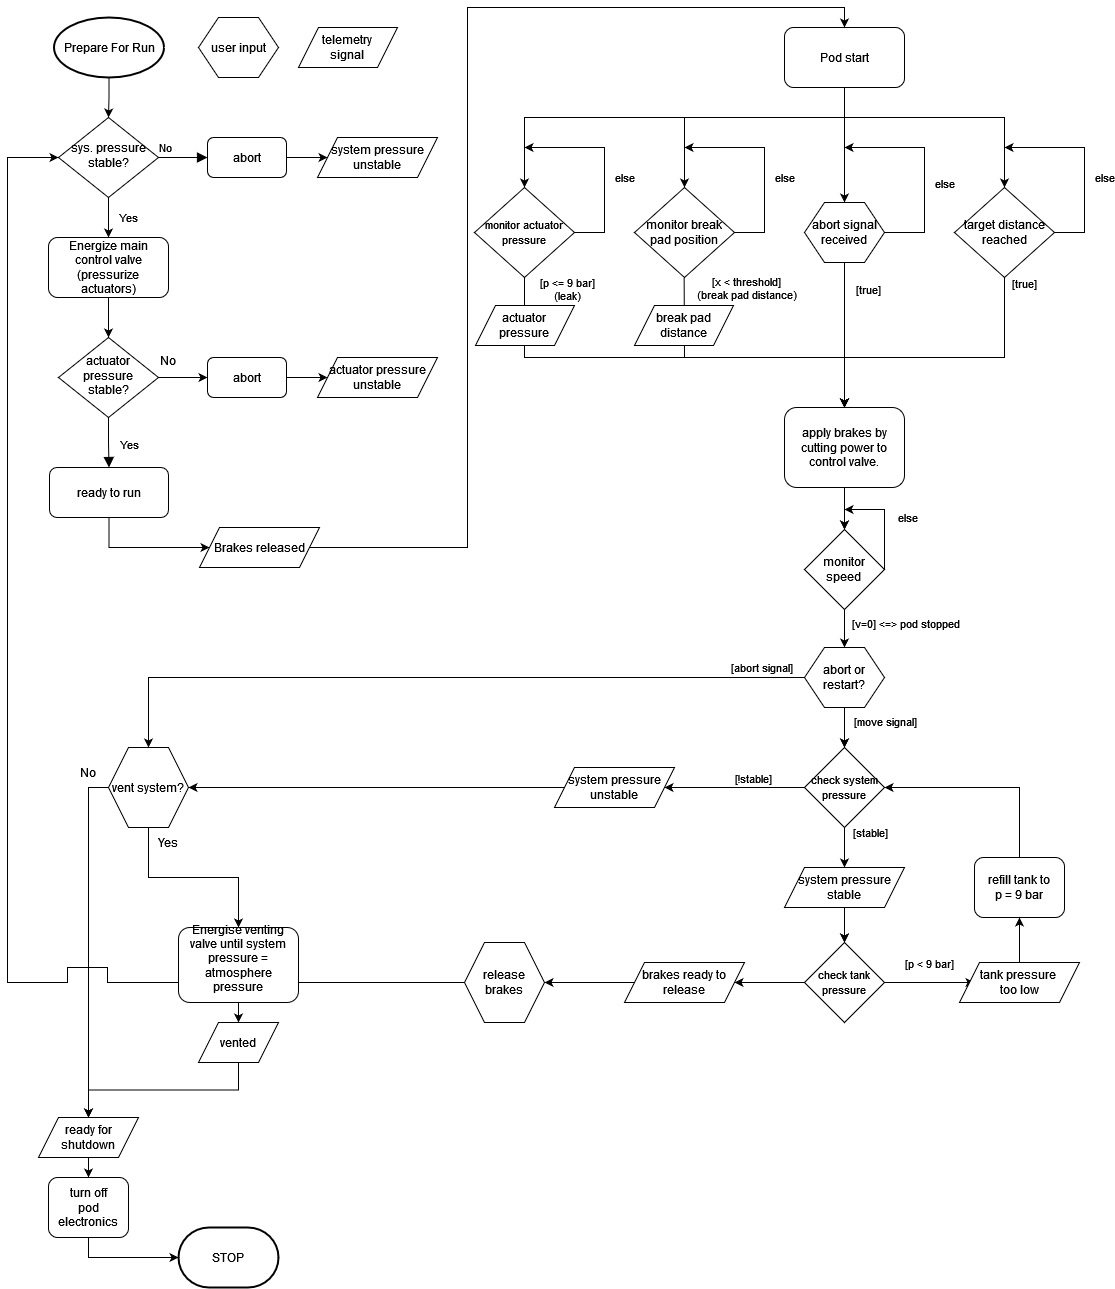
\includegraphics[width=\textwidth]{texfiles/elec/eimg/brakesoftware_ext}
The implementation of the hardware architecture goes as follows:
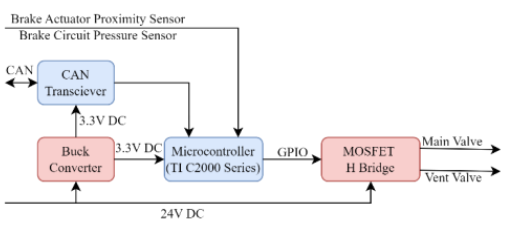
\includegraphics[width=\textwidth]{texfiles/elec/eimg/Brakes_architecture}

\subsubsection{Thermal Controller}
it follows the following state diagram: \\
\textbf{--- INSERT STATE DIAGRAM ---}
%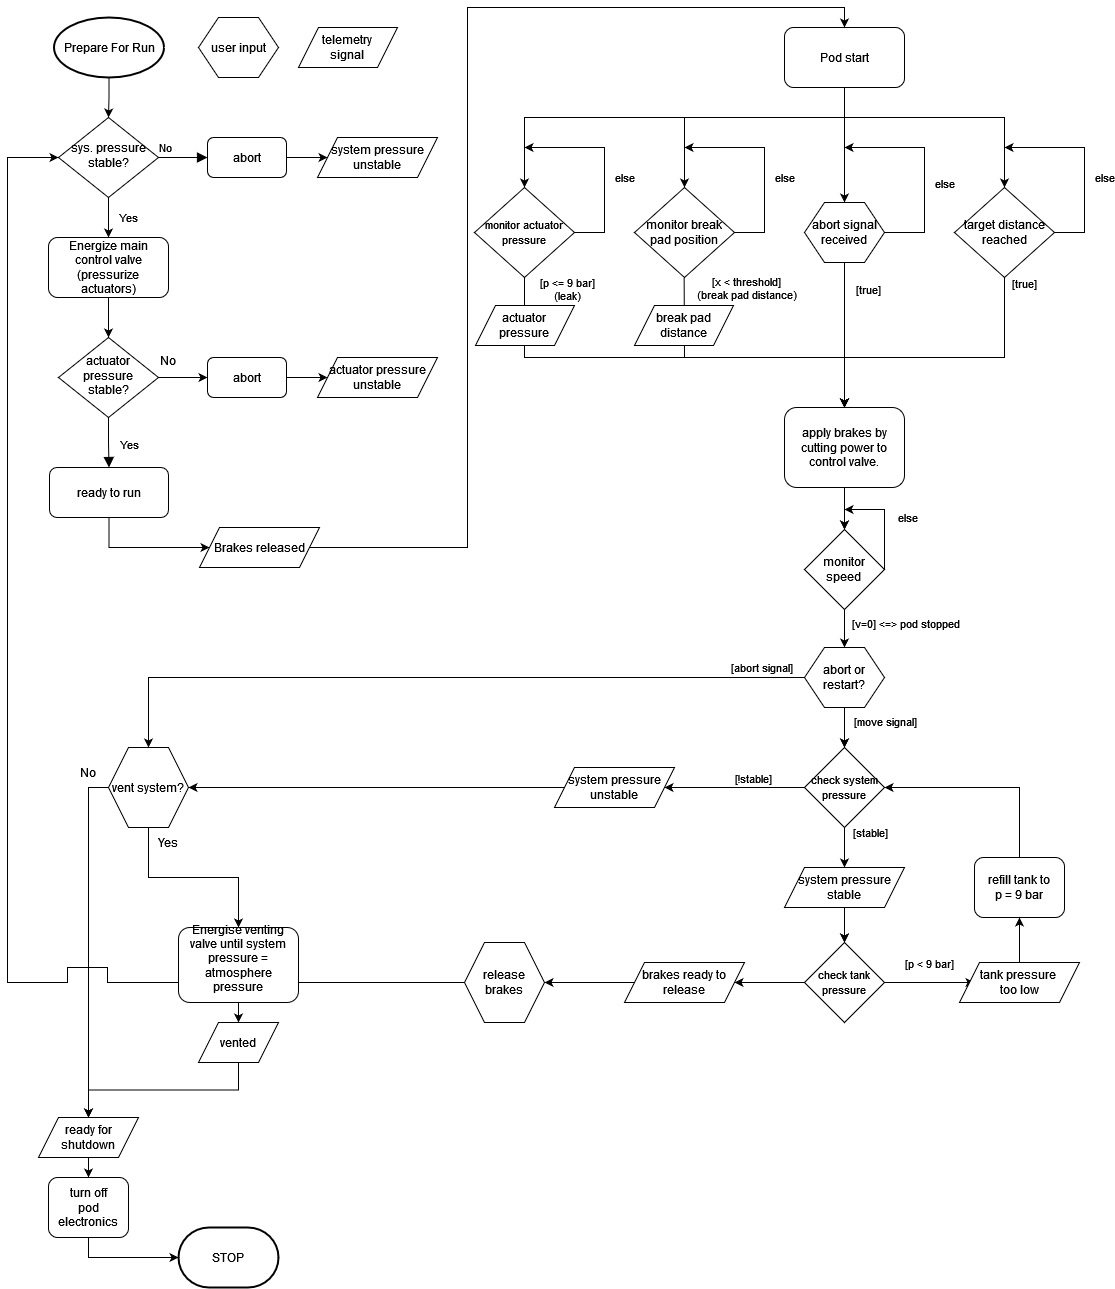
\includegraphics[width=\textwidth]{texfiles/elec/eimg/brakesoftware_ext}

The following hardware architecture is to be implemented:
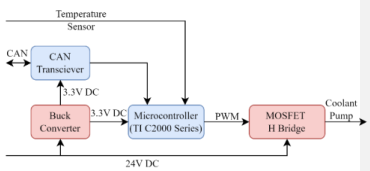
\includegraphics[width=\textwidth]{texfiles/elec/eimg/Thermal_architecture}

\subsection{Control Boards/Units in the Vehicle}
% Insert content from the first snippet related to Control Boards/Units in the Vehicle here.

\begin{enumerate}
    \item Brakes Controller
    Lacking. To be added.

    \item Thermal Controller
The Thermal Management Controller is responsible for cooling the Traction Components, i.e., Motor and Traction Controller. The actuator is the coolant pump which is controlled  with the feedback of the temperature of coolant in the cooling loop.  The Pump Speed is controlled via PWM to the MOSFET Bridge. The PWM duty cycle is simply calculated from a lookup table that is referenced to the temperature difference between target and actual temperatures. The only safety feature to be developed is to issue an emergency stop signal to HV Systems in the event the coolant temperature exceeds a critical
temperature.

\end{enumerate}

\subsubsection{Parts List}

\begin{table}[H]
\centering
\begin{tabular}{|l|l|l|}
\hline
\textbf{Part} & \textbf{Manufacturer} & \textbf{Description} \\ \hline
Raspberry Pi Zero 2 W & Raspberry & Microcontroller for telemetry \\ \hline
Raspberry Pi 4 B & Raspberry & Computer for telemetry \\ \hline
MC3479 & Memsic & 3-Axis Accelerometer \\ \hline
RS485 CAN HAT & Waveshare & CAN adapter for RPI4B \\ \hline
\end{tabular}
\caption{Telemetry System Parts List}
\label{tab:my-table}
\end{table}



\subsection{Integration with other systems}
The friction brakes, the cooling pump and the motor are controlled through our system.

\subsection{Graphical User Interface (GUI)}
% Insert content from the first snippet related to GUI here.

% Continue merging additional sections and sub-sections from the first snippet into the structured format of the second snippet as needed.

\subsection{Telemetry Device}
For communication and navigation, we use our telemetry system, that consists of a CAN bus, a CAN2WLAN transmitter and a VCU.
\subsubsection{Introduction}
\begin{enumerate}
    \item Brief overview of Telemetry Components
    \item Diagram with the connection of all boards with NAP and control station.
    \item Explanation of the Signals Transmitted
\end{enumerate}

\subsubsection{Parts Lists}